\section{Installazione}\label{Installazione}

\subsection{Requisiti}\label{Requisiti}
I requisiti minimi richiesti per il funzionamento del plug-in non sono dovuti al prodotto in sè, ma sono dovuti alle tecnologie che vengono utilizzate. Pertanto si rimanda ai requisiti minimi delle seguenti tecnologie:
\begin{itemize}
	\item \textit{InfluxDB};
	\item \textit{Grafana};
	\item \textit{NodeJS}; 
	\item \textit{pm2}. 
\end{itemize}

\subsubsection{Installazione plug-in}
Viene richiesta come pre-condizione l'installazione di grafana a seconda del sistema operativo utilizzato seguendo la documentazione fornita da quest'ultima. 
\begin{enumerate}
	\item Arrestare l'esecuzione di \textit{Grafana}, qualora fosse in esecuzione;	
	\item Copiare la directory del progetto all'interno della cartella predestinata da \textit{Grafana} per ospitare i plug-in aggiuntivi da installare.
	\item Per poter utilizzare il prodotto all'interno di \textit{Grafana}, e poiché quest'ultimo sia riconosciuto come plug-in, è necessario per prima cosa eseguire la build del prodotto.
	La build del prodotto avviene attraverso due fasi: la prima che va a risolvere le dipendenze, la seconda che esegue la build.\\
	Il processo di build avviene attraverso l'intervento del module bundler \textit{WebPack}.
	È necessario quindi eseguire i seguenti comandi dalla directory che ospita il plug-in:
\begin{center}
	\texttt{npm install}\\
	\texttt{npm run build}
\end{center}
\item Avviare \textit{Grafana} e procedere all'aggiunta del plug-in.
Per informazioni relative al funzionamento del plug-in si rimanda al \textit{Manuale Utente v1.0.0}.
\end{enumerate}

\subsubsection{Installazione server}\label{installazione_server}
\paragraph{Installazione NodeJS}
	\begin{itemize}
		\item Scaricare l'ultima versione di NodeJS LTS\glossario dal sito ufficiale; 
		\begin{figure}[H]
		\begin{center}
			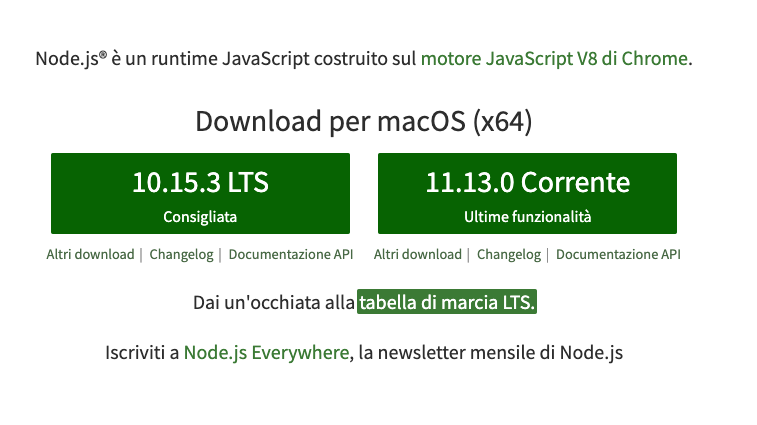
\includegraphics[scale=0.5]{./images/nodejs.png} 
		\end{center}
		\caption{Selezione versione NodeJS}
	\end{figure}
	\item Installare NodeJS; 
		\begin{figure}[H]
		\begin{center}
			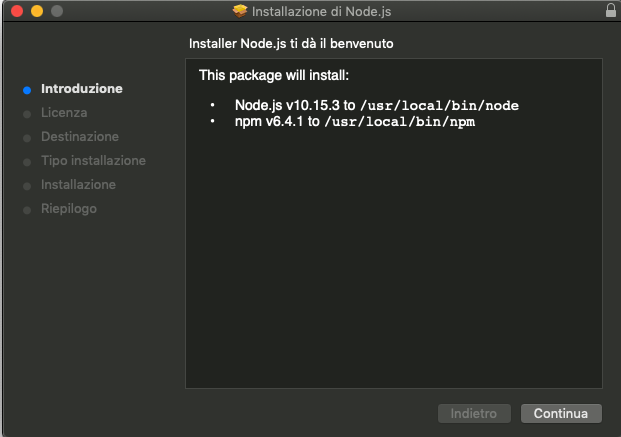
\includegraphics[scale=0.5]{./images/install_nodejs.png} 
		\end{center}
		\caption{Installazione NodeJS}
	\end{figure}	
	\end{itemize}

\paragraph{Installazione pm2}
\begin{itemize}
	\item Aprire un terminale nel S.O. dove si intente eseguire il server; 
	\item Installare globalmente il modulo \texttt{pm2} tramite il gestore di pacchetti \texttt{npm}, usando il seguente commando: 
	\begin{center}
		\texttt{npm install pm2 -g}
	\end{center}
\end{itemize}
		


	
	
\subsection{Esecuzione}\label{run}
\subsubsection{Esecuzione plug-in}
\begin{itemize}
	\item Aprire il browser consigliato; 
	\item Collegarsi all'indirizzo ip di grafana sulla porta 3000 (le configurazione di default suggeriscono \texttt{http://localhost:3000}); 
	\item Accedere al sistema con le credenziali pre-impostate; 
	\item Nella dashboard selezionata, aggiungere il pannello \textit{"GrafanaAndBayes"}; 
	\item Accedere alle impostazioni del plug-in inserendo l'indirizzo ip e la porta del server in ascolto. 
\end{itemize}


\subsubsection{Esecuzione server}
\begin{itemize}
	\item Aprire un terminale e spostarsi nella directory contenente il server; 
	\item Da terminale, eseguire il seguente commando il quale avvia il server attraverso il manager dei processi pm2
	\begin{center}
		\texttt{pm2 start ./src/index.js --- -p :porta}
	\end{center}
	dove \textbf{:porta} e il numero della porta su cui impostare il server in ascolto; 
\end{itemize}
	
	
	
	
	
	
	
	
	
	
	
	
	
	
	
	
	
	
	
	
	